% TrafficSense: IEEE conference paper (condensed from docs/report).
%
% Every number from the data is written \V{key}{number}: \V prints the number and ignores the
% key, which names a fact read from outputs/ (src/trafficsense/report/facts.py) or a cell of a
% checked table. Tables between "% BEGIN:name" and "% END:name" are generated.
%   python scripts/make_paper.py           # refresh tables, figures, numbers; build PDF and zip
%   python scripts/make_paper.py --check   # fail if anything differs from outputs/
% Do not type a result number without a tag: the check fails on it.
%
\documentclass[conference]{IEEEtran}
\IEEEoverridecommandlockouts
\usepackage{iftex}
\ifPDFTeX
  \usepackage[T1]{fontenc}
\fi
\usepackage{newtxtext,newtxmath}
\usepackage{graphicx}
\usepackage{booktabs}
\usepackage{amsmath}
\usepackage{cite}
\usepackage{url}

\newcommand{\V}[2]{\ensuremath{#2}}
\newcommand{\EmailA}{\texttt{bhargav.23bce8195@vitapstudent.ac.in}}
\newcommand{\EmailB}{\texttt{akul.23bce8015@vitapstudent.ac.in}}
\newcommand{\EmailC}{\texttt{amit.23bce8288@vitapstudent.ac.in}}
\newcommand{\EmailD}{\texttt{abhishek.23bce9470@vitapstudent.ac.in}}
\newcommand{\CapstoneID}{3328F4C8}
\newcommand{\model}[1]{\texttt{#1}}

\begin{document}

\title{TrafficSense: An AI-Based Smart Traffic Management System\\
{\large Guarded Local-LLM Signal Control, Ambulance Priority and Camera Errors on an Indian Road Network}%
\thanks{B.Tech CSE and Specializations, Capstone Project, Fall 2026-27, Capstone ID \CapstoneID.
Registration numbers: C Bhargav Kumar 23BCE8195, Achalla Akul Lakhan 23BCE8015,
Darsi Amit 23BCE8288, Mylapalli Abhishek Raj 23BCE9470.}}

\newcommand{\authorbox}[3]{\begin{minipage}[t]{#1}\centering
{\normalsize #2}\\
\textit{\small School of Computer Science}\\
\textit{\small and Engineering, VIT-AP University}\\
{\small Amaravati, India}#3
\end{minipage}}
\newcommand{\emailline}[1]{\\{\footnotesize #1}}

\author{
\IEEEauthorblockA{%
\authorbox{0.31\textwidth}{C Bhargav Kumar}{\emailline{\EmailA}}\hfill
\authorbox{0.31\textwidth}{Achalla Akul Lakhan}{\emailline{\EmailB}}\hfill
\authorbox{0.31\textwidth}{Darsi Amit}{\emailline{\EmailC}}\\[1.5ex]
\authorbox{0.38\textwidth}{Mylapalli Abhishek Raj}{\emailline{\EmailD}}\hspace{0.08\textwidth}
\authorbox{0.38\textwidth}{Dr.\ Mohd Irfan (Guide)}{}}
}

\maketitle

\begin{abstract}
Signalised junctions in Indian cities carry a mixed stream of two-wheelers, auto-rickshaws,
cars, buses and trucks, and many still run fixed plans that give emergency vehicles no
priority. Large language models (LLMs) have been proposed as signal agents that can use
context such as an approaching ambulance. We ask whether such agents, running a small model on
a 4 GB laptop GPU, can match the best classical controller, and how they cope with counts from
a real camera detector. TrafficSense places one LLM agent at each intersection of a CityFlow
network, adapted from CoLLMLight; our pipeline reproduces the CoLLMLight authors' baseline
results within the simulator's run-to-run noise. On a calibrated 2x2 network with an Indian
vehicle mix, with MaxPressure and a Webster plan tuned first and the evaluation pre-registered,
the selected controller (\model{llama3.2:3b}, guided and guarded by MaxPressure) matched
MaxPressure's average travel time to within \V{f.peak.llm.vs_mp}{0.5}--\V{f.off.llm.vs_mp}{0.9}\%
but did not improve on it. With ambulances listed in its prompt, their mean travel time fell
from \V{e.mp.amb}{130.1}~s to \V{e.llm.amb}{88.9}~s, close to rule-based preemption
(\V{e.pre.amb}{81.2}~s), at no measurable cost to other traffic. A YOLOv8n detector trained on
the India Driving Dataset reached mAP50 \V{d.test.map50}{0.563} on held-out drives; its
measured errors, injected into the controllers' counts, raised MaxPressure's travel time by
\V{c.peak.mp.junction.pct}{2.3}--\V{c.off.mp.junction.pct}{4.8}\%, mainly through false
detections, while the fixed plan was unaffected. A small LLM agent is therefore best used as a
guarded layer that adds context MaxPressure cannot use, not as its replacement.
\end{abstract}

\begin{IEEEkeywords}
traffic signal control, large language models, multi-agent systems, MaxPressure, emergency
vehicle priority, YOLOv8, India Driving Dataset, CityFlow, pre-registration
\end{IEEEkeywords}

\section{Introduction}

Indian urban traffic differs from the traffic most signal-control methods were built for.
Two-wheelers and three-wheelers dominate the stream: in the Chennai modal share used for our
scenario~\cite{itrans2009}, motorised two-wheelers are
\V{docs/indian_scenario.md | mix | motorcycle | Share (config}{45.1}\% of vehicles. Lane
discipline is weak, so per-lane loop detectors work poorly~\cite{mathew2010calibration}, and
capacity depends on the vehicle mix~\cite{chandra2003lanewidth,indohcm2017}. Many junctions
still run fixed plans, and ambulances wait at red signals with no priority system.

Classical controllers range from fixed-time plans~\cite{webster1958} to
MaxPressure~\cite{varaiya2013maxpressure}, which needs no training and has a stability proof.
Since 2023, LLMs have been tried as signal agents~\cite{lai2023llmlight,wang2024lalight}.
CoLLMLight~\cite{yuan2026collmlight}, the base paper of this work, places one LLM agent at each
intersection and lets neighbours cooperate through the prompt. The appeal is not optimisation
power but context: an agent can be told in words that an ambulance is approaching. Published
LLM controllers, however, are usually evaluated with large or fine-tuned models, against
baselines not tuned for the test network, and on exact simulator counts.

We test a small \emph{local} model, without fine-tuning, under a pre-registered plan. Our
contributions are:
\begin{itemize}
\item a simulation pipeline validated against CoLLMLight's own code, which also exposed a bug
  in its fixed-time baseline (Section~\ref{sec:validation});
\item a pre-registered comparison of guarded LLM controllers with a tuned MaxPressure and a
  Webster plan on an Indian-mix network: the selected controller matches MaxPressure but does
  not beat it, and its decision logs show why (Section~\ref{sec:res-main});
\item a clear benefit for ambulances: listing them in the prompt cuts their mean travel time
  by \V{e.llm.amb_cut_vs_mp}{31.7}\% against MaxPressure (Section~\ref{sec:res-amb});
\item a camera-error study in which errors measured on Indian street images degrade the
  controllers' counts, with a post-hoc decomposition by error type (Section~\ref{sec:res-cam});
\item every number in this paper is generated from, or checked by a script against, the
  result files.
\end{itemize}

\section{Related Work}

\textbf{Fixed-time and adaptive control.} Webster's method~\cite{webster1958} gives the
delay-minimising cycle of a fixed plan from flow ratios. Adaptive systems such as
SCATS~\cite{sims1980scat} and SCOOT~\cite{hunt1981scoot} adjust plans from dense detector
networks, which are rare on Indian roads.

\textbf{MaxPressure.} Back-pressure scheduling stabilises a queueing network whenever any policy
can~\cite{tassiulas1992}; Varaiya carried it to traffic signals~\cite{varaiya2013maxpressure}.
The pressure of a phase $p$ is $P(p)=\sum_{(l,m)\in p}(x_l-x_m)$, with $x$ the queued vehicles on
incoming lane $l$ and outgoing lane $m$; the phase with the highest pressure gets green.

\textbf{Reinforcement learning} (RL) learns a phase policy in simulation~\cite{wei2021survey}:
IntelliLight~\cite{wei2018intellilight}, PressLight~\cite{wei2019presslight},
CoLight~\cite{wei2019colight} and MPLight~\cite{chen2020mplight}, mostly on
CityFlow~\cite{zhang2019cityflow}. RL needs long training per network and does not explain its
decisions.

\textbf{LLM agents.} LLMLight~\cite{lai2023llmlight} prompts an LLM with one intersection's
state; LA-Light~\cite{wang2024lalight} gives it tools for rare events such as emergencies.
CoLLMLight~\cite{yuan2026collmlight} adds cooperative reasoning over neighbours, an asynchronous
decision architecture and cost-aware fine-tuning. We keep its multi-agent structure, its
neighbour information and its datasets, but not its training.

\textbf{Vision-based sensing.} Cameras are the usual sensor for mixed
traffic~\cite{buch2011review}; YOLO detectors~\cite{redmon2016yolo,jocher2023yolov8} run in real
time on modest hardware, and visual sensing has been proposed for ambulance
priority~\cite{nellore2016emergency}. The India Driving Dataset (IDD)~\cite{varma2019idd}
covers Indian classes such as auto-rickshaws. Detection papers report mAP~\cite{lin2014coco};
a controller is hurt instead by errors in its \emph{counts}, which we measure.

\section{Method}

\subsection{System overview}
Fig.~\ref{fig:overview} shows the system. CityFlow holds the exact state and is the only place
where metrics are measured. Controllers read lane counts through an observation layer that
returns exact counts or, in the camera experiment, counts degraded by measured detector errors.
Every run writes its provenance (controller, model as reported by the server, seed, scenario,
git commit, LLM calls, failures and latency) to its result files.

\begin{figure}[t]
\centering
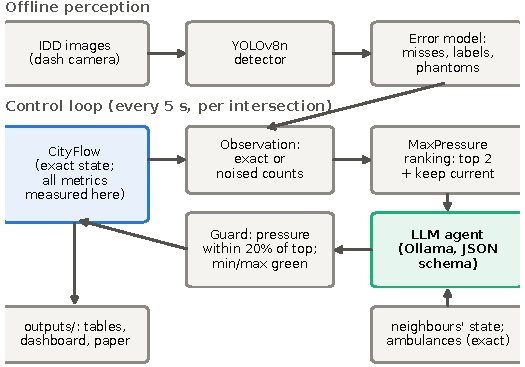
\includegraphics[width=\columnwidth]{figures/overview.pdf}
\caption{System overview. Controllers see the simulator only through the observation layer;
ambulance positions reach the agent through a separate, exact channel.}
\label{fig:overview}
\end{figure}

\subsection{Per-junction LLM agent loop}
Every \V{cfg.mp.interval}{5}~s, each intersection whose green has lasted its minimum is asked
for its next phase. (1)~\emph{Observe}: a short prompt gives, for each phase offered, its
pressure and queue, so no arithmetic is needed, and for each neighbour its current phase and
the stopped vehicles heading towards this junction. (2)~\emph{Reason}: the prompt goes to a
local model through Ollama's \texttt{/api/chat}~\cite{ollama} with a JSON schema that restricts
the answer to the offered phases and a short reason, at temperature 0 with a fixed seed.
(3)~\emph{Act}: the answer is validated (phase offered, reason of at most
\V{code.reason_words.guided_v3}{15} words); a failure is counted by type and MaxPressure's
choice is applied for that decision. (4)~\emph{Enforce}: the wrapper inserts the 5~s transition
and applies a \V{cfg.mp.min_green}{15}~s minimum and \V{cfg.signal.max_green}{60}~s maximum
green. (5)~\emph{Log}: state, raw answer, latency and applied phase are written per decision.
All agents share one GPU, so the decision interval must fit one call per intersection.

\subsection{Controller arms}
\emph{Plain} arms let the LLM choose any green phase. \emph{Hybrid} arms offer MaxPressure's two
best phases or keeping the current one. The \emph{guarded} arm also applies the LLM's choice
only if its pressure is close to the best,
$P \ge P_{\mathrm{top}} - (1-r)\,|P_{\mathrm{top}}|$ with $r=\V{cfg.guard.ratio}{0.8}$, i.e.\
within \V{cfg.guard.margin}{20}\% of the top pressure; otherwise MaxPressure's choice is applied
and the override counted. The guard was added after early rounds showed small models choosing
low-pressure phases.

\subsection{Ambulance handling}
An ambulance within \V{cfg.amb.range}{150}~m of the stop line is listed in the prompt with its
movement, distance and serving phases, and the system prompt adds one sentence asking for green
for it. A serving phase is added to the options if none is offered, and is exempt from the
guard. The non-LLM competitor is MaxPressure with preemption: the serving phase with the highest
pressure gets green, within the same green limits. Ambulance positions are assumed to come from
GPS or V2X and are never noised.

\subsection{Perception error model}\label{sec:perc}
We trained YOLOv8n~\cite{jocher2023yolov8} on IDD with 7 classes (car, motorcycle,
auto-rickshaw, bus, truck, bicycle, person) at \V{cfg.imgsz}{640}~px, splitting by drive so
that near-duplicate frames cannot leak; IDD's official validation split is our test split,
used once after the confidence threshold (\V{d.conf}{0.3}, maximum mean F1 on validation) was
frozen. Detections are matched to ground truth at IoU $\ge$ \V{d.match_iou}{0.5}, class-free;
the measured rates become the error model: a per-class detection probability, label
probabilities from the confusion matrix, and a Poisson number of phantom stopped vehicles per
road and snapshot. The \emph{junction} level uses detection rates of medium and large objects
(queued vehicles near a pole camera); the \emph{crowded / far} level uses all objects. A fresh
snapshot is drawn at every observation, while the simulator stays exact.

\section{Experimental Setup}

\subsection{Simulator validation}\label{sec:validation}
CoLLMLight's FixedTime and MaxPressure were run unmodified, and our environment was driven the
same way (4 phases, a decision every \V{val.matched.interval}{30}~s, the same CityFlow seed).
Scored with their metric definitions, throughput, queue length and waiting time were identical
floating-point numbers on all three of their datasets; average travel time differed at most in
the sixth significant digit, within CityFlow's own run-to-run noise with lane changing on. The
check exposed a bug: their fixed-time agent computes \texttt{(cur\_phase+1)\%4} on a 1-based
phase, so it alternates between the two east--west phases and north--south traffic never gets
green. We use only our own, correct fixed-time controllers.

\subsection{Indian 2x2 scenario}
A 2x2 grid with \V{scn.roadnet.spacing_m}{200}~m links and three lanes per approach carries five vehicle types (motorcycle,
auto-rickshaw, car, bus, truck) with Indian dimensions~\cite{umapathi2019pcu} and the Chennai
modal share~\cite{itrans2009}, arriving as Poisson flows; each seed is a different flow file.
CityFlow is lane-based, so the scenario models the Indian \emph{mix} but not lane-free driving.
Demand was calibrated by a rule fixed in advance: under MaxPressure, the lowest swept demand
that does not drain is $R^*=\V{cal.r_star}{5500}$~veh/h; peak is the largest draining demand
at or below $\V{cal.rule.peak_fraction}{0.9}R^*$, \V{cal.peak}{4750}~veh/h, and off-peak half of
it, \V{cal.offpeak}{2375}~veh/h. We also use CoLLMLight's Jinan 3x4 network with its real flow.

\subsection{Baselines}
FixedTime gives each of 4 paired phases \V{cfg.ft.green}{30}~s. The Webster plan computes cycle
and splits per intersection from saturation flows measured in the simulator and the run's own
flow file, a perfect count that favours it. MaxPressure's minimum green was tuned before any LLM
run with a pre-registered rank rule over four scenarios; it chose \V{mg.chosen}{15}~s.

\subsection{LLM selection and pre-registration}
Each arm was benchmarked on the first \V{b.steps}{600}~s of Indian peak traffic with
\model{llama3.2:3b}~\cite{grattafiori2024llama3}, \model{qwen2.5:3b}~\cite{qwen2024qwen25}
and Google's \model{gemma4:e4b} (\model{gemma3:4b} in the first round only; it did not fit in
4 GB). The pre-registered rule makes a model eligible if fewer than
\V{b.rule.fail_pct}{2}\% of its calls fail and its 95th-percentile latency is below
\V{b.rule.p95_s}{3}~s, then picks the lowest mean queue. After the final, pre-registered round
it selected the guarded arm with \model{llama3.2:3b} and a 5~s decision interval. The
\model{gemma4:e4b} hybrid, which failed the rule only on latency (p95
\V{b.hybrid_v3.gemma4:e4b.p95}{4.80}~s), was added to the full runs as an \emph{exploratory}
arm. Prompt v3, which states that higher pressure means a phase needs green more, was a
post-hoc fix after earlier rounds; a model-size study and the camera decomposition are also
exploratory or post-hoc. All four are labelled wherever they appear~\cite{nosek2018prereg}.

\subsection{Runs and metrics}
Every run is \V{cfg.steps}{3600}~s; Indian off-peak, peak and Jinan use seeds 0--2 and the
emergency scenario seeds 0--4. The full experiments comprise \V{f.runs}{67} runs and the camera
experiment \V{c.runs}{130}. The primary metric is the average travel time (ATT) from CityFlow,
which includes time spent waiting to enter the network. We also measure queue length (vehicles
below \V{code.stop_speed}{0.1}~m/s on incoming lanes) and, for ambulances, travel time per
signal-relevant ambulance. Results are mean $\pm$ sample standard deviation over seeds; the most
informative comparison is paired by seed. With 3 seeds (5 with ambulances) no significance test
was pre-registered; a difference counts only if it has the same sign on every seed and is large
against the seed spread. Repeated baseline runs were identical in
\V{f.reproduced}{27} of \V{f.reproduced_of}{27} cases.

\section{Results}

\subsection{Main comparison}\label{sec:res-main}
Table~\ref{tab:main} and Fig.~\ref{fig:paired} give the full experiments. The pre-registered
controller's ATT is \V{f.off.llm.vs_mp}{+0.9}\% (off-peak), \V{f.peak.llm.vs_mp}{+0.5}\%
(peak) and \V{f.jinan.llm.vs_mp}{+0.8}\% (Jinan) relative to MaxPressure, and it is behind on
\V{p.off.llm.higher}{3} of 3 off-peak, \V{p.peak.llm.higher}{2} of 3 peak and
\V{p.jinan.llm.higher}{3} of 3 Jinan seeds. Its own answer differs from MaxPressure's in
\V{l.amb.llm.differs}{87}--\V{l.peak.llm.differs}{93}\% of calls, the guard replaces
\V{l.amb.llm.guard}{76}--\V{l.peak.llm.guard}{83}\% of calls, and the applied phase differs
in only \V{l.peak.llm.applied}{10}--\V{l.jinan.llm.applied}{11}\%. It never failed a call
off-peak or at peak and runs in real time (\V{l.peak.llm.lat}{1.02}--\V{l.jinan.llm.lat}{1.10}~s
per call). At peak, MaxPressure and the Webster plan are themselves level.

The exploratory \model{gemma4:e4b} arm is the only LLM arm faster than MaxPressure anywhere:
at peak, on all \V{p.peak.gem.lower}{3} seeds (\V{f.peak.gem.vs_mp}{-1.5}\% on the mean),
while off-peak it is slower on every seed (\V{f.off.gem.vs_mp}{+2.7}\%). With three seeds this
is a lead, not a demonstrated gain, and at \V{l.peak.gem.lat}{4.54}~s per call it is not real
time on this GPU.

\begin{table}[t]
\caption{Average travel time (s), mean $\pm$ std over seeds 0--2, \V{cfg.steps}{3600}~s runs.}
\label{tab:main}
\centering
\footnotesize
% BEGIN:tab_main
\begin{tabular}{@{}lccc@{}}
\toprule
Controller & Off-peak & Peak & Jinan 3x4 \\
\midrule
FixedTime, 30\,s & $121.5 \pm 0.2$ & $279.9 \pm 9.9$ & $423.0 \pm 0.0$ \\
Webster plan & $100.4 \pm 4.1$ & $116.3 \pm 4.6$ & $416.1 \pm 0.0$ \\
MaxPressure (tuned) & $88.1 \pm 1.0$ & $115.5 \pm 0.9$ & $300.9 \pm 0.0$ \\
\midrule
LLM guarded$^{a}$ & $89.0 \pm 0.8$ & $116.1 \pm 2.9$ & $303.2 \pm 1.1$ \\
LLM hybrid$^{b}$ & $90.5 \pm 1.2$ & $113.7 \pm 0.3$ & -- \\
\bottomrule
\end{tabular}
% END:tab_main
\par\vspace{2pt}
\parbox{\columnwidth}{\scriptsize $^{a}$Pre-registered: guarded hybrid, \model{llama3.2:3b}.
$^{b}$Exploratory, not selected by the rule: hybrid, \model{gemma4:e4b}; not run on Jinan.
Off-peak \V{cal.offpeak}{2375}, peak \V{cal.peak}{4750} veh/h. Jinan's flow file is fixed, so
the deterministic baselines do not vary.}
\end{table}

\begin{figure}[t]
\centering
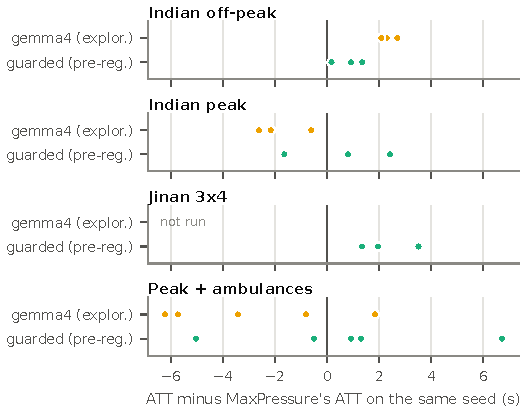
\includegraphics[width=\columnwidth]{figures/paired.pdf}
\caption{ATT of each LLM arm minus MaxPressure's ATT on the same seed; each dot is one seed,
left of zero is faster than MaxPressure.}
\label{fig:paired}
\end{figure}

\subsection{Ambulances}\label{sec:res-amb}
Ambulances arrive at \V{scn.emergency.veh_per_hour}{6} per hour on top of peak traffic; over 5
seeds, \V{e.mp.amb_n}{29} of the \V{e.mp.amb_all_n}{37} ambulances cross a signalised movement.
Both LLM arms get most of the benefit of preemption (Table~\ref{tab:amb},
Fig.~\ref{fig:amb}): mean travel time is \V{e.mp.amb}{130.1}~s under MaxPressure,
\V{e.llm.amb}{88.9}~s under the pre-registered arm and \V{e.pre.amb}{81.2}~s with preemption.
The gain is almost all time no longer spent stopped (\V{e.mp.amb_stop}{62.3}~s against
\V{e.llm.amb_stop}{21.2}~s). Paired by ambulance, the main arm is \V{e.llm.vs_pre}{7.7}~s
slower than preemption on average. Network ATT, \V{e.llm.att}{116.4}~s against MaxPressure's
\V{e.mp.att}{115.7}~s, is well inside the seed spread ($\pm$\V{e.mp.att_sd}{2.3}~s).

\begin{table}[t]
\caption{Signal-relevant ambulances, pooled over seeds 0--4, and network ATT (mean $\pm$ std); all in seconds.}
\label{tab:amb}
\centering
\footnotesize
% BEGIN:tab_ambulance
\begin{tabular}{@{}lcccc@{}}
\toprule
Controller & Amb.\ TT & Stopped & vs preempt. & Network ATT \\
\midrule
MaxPressure & $130.1$ & $62.3$ & $+48.9$ (1/28) & $115.7 \pm 2.3$ \\
Webster plan & $123.5$ & $55.0$ & $+42.3$ (4/25) & $115.2 \pm 2.7$ \\
MP + preemption & $81.2$ & $14.1$ & -- & $116.0 \pm 0.7$ \\
LLM guarded$^{a}$ & $88.9$ & $21.2$ & $+7.7$ (12/15) & $116.4 \pm 3.1$ \\
LLM hybrid$^{b}$ & $82.2$ & $15.3$ & $+1.1$ (16/12) & $112.9 \pm 1.9$ \\
\bottomrule
\end{tabular}
% END:tab_ambulance
\par\vspace{2pt}
\parbox{\columnwidth}{\scriptsize Amb.\ TT: mean ambulance travel time; vs preempt.: mean
paired difference to the same ambulance under preemption (faster/slower count).
$^{a,b}$As in Table~\ref{tab:main}.}
\end{table}

\begin{figure}[t]
\centering
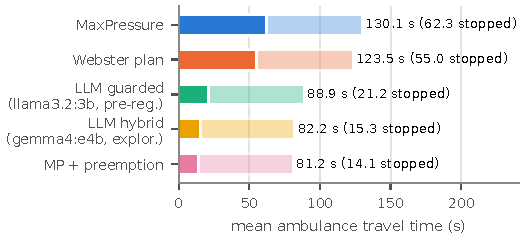
\includegraphics[width=\columnwidth]{figures/ambulance.pdf}
\caption{Mean travel time of the signal-relevant ambulances; solid part = time stopped.}
\label{fig:amb}
\end{figure}

\subsection{Model size (exploratory)}
Keeping the unguarded hybrid and changing only the model, both 3~B models made it far worse
than MaxPressure on every seed (\V{m.peak.qwen.vs_mp}{+51.0}\% and
\V{m.peak.llama3b.vs_mp}{+81.4}\% at peak). \model{gemma4:e4b}, \model{llama3.1:8b} and a
hosted \V{m.size.nemo}{550}~B mixture-of-experts model~\cite{nemotron3ultra} were within seed
noise of MaxPressure (the hosted API throttled heavily; \V{m.peak.nemo.fail}{1.8}\% of its calls failed
and fell back to MaxPressure's choice); they chose the highest-pressure option in \V{m.peak.gem.follows}{80},
\V{m.peak.llama8b.follows}{62} and \V{m.peak.nemo.follows}{99}\% of calls.

\subsection{Camera errors}\label{sec:res-cam}
The detector reaches mAP50 \V{d.test.map50}{0.563} and mAP50-95 \V{d.test.map5095}{0.375} on
the test split, with high precision and moderate recall; it misses
\V{d.size.motorcycle.small}{59}--\V{d.size.person.small}{76}\% of small objects but only
\V{d.size.autorickshaw.large}{1}--\V{d.size.bicycle.large}{22}\% of large ones.
With its errors in the counts (Table~\ref{tab:cam}), MaxPressure's ATT rises by
\V{c.off.mp.junction.pct}{4.8}\% off-peak and \V{c.peak.mp.junction.pct}{2.3}\% at peak with
the junction camera, worse on every seed; the LLM arm degrades about as much, since its guard
reads the same counts; the Webster plan, which reads no counts, is unaffected. At peak,
MaxPressure (\V{c.peak.mp.junction.att}{118.2}~s) falls behind Webster
(\V{c.peak.web.junction.att}{116.3}~s).

Misses alone cost little (Fig.~\ref{fig:cam}b): with half of all vehicles missed and no
phantoms, MaxPressure loses \V{c.sweep.off.p50.pct}{3.0}\% off-peak, because uniform misses
shrink every pressure by the same factor. The junction camera detects
\V{c.peff.off.junction.pct}{92}\% of vehicles yet costs \V{c.off.mp.junction.pct}{4.8}\%,
against \V{c.sweep.off.p90.pct}{0.0}\% for \V{c.sweep.off.p90.level_pct}{90}\% detection
without phantoms; it adds about \V{c.phantoms_per_road}{0.7} phantom stopped vehicles per road
and snapshot. A post-hoc decomposition (Fig.~\ref{fig:cam}a) confirms it off-peak: false
detections alone cost \V{c.dec.false.off.pct}{+3.8}\% of the \V{c.dec.all.off.pct}{+4.8}\%.
At peak the components sum to only \V{c.dec.sum.peak.pct}{+0.4}\% of
\V{c.dec.all.peak.pct}{+2.3}\%; three seeds cannot tell interaction from chance. With
junction-camera counts the LLM arm's ambulances were \V{c.amb.llm.junction.amb_d}{11.0}~s slower
on average, not distinguishable from zero with \V{e.mp.amb_n}{29} ambulances; preemption,
reading the exact channel, kept its advantage.

\begin{table}[t]
\caption{ATT change against perfect counts, paired by seed: mean \% [seed range].}
\label{tab:cam}
\centering
\footnotesize
\setlength{\tabcolsep}{2.5pt}
% BEGIN:tab_camera
\begin{tabular}{@{}l@{\hspace{4pt}}cccc@{}}
\toprule
 & \multicolumn{2}{c}{Off-peak} & \multicolumn{2}{c}{Peak} \\
\cmidrule(lr){2-3}\cmidrule(l){4-5}
Controller & junction & crowded & junction & crowded \\
\midrule
MaxPressure & $+4.8$ {\scriptsize[$4.1$, $5.4$]} & $+8.2$ {\scriptsize[$7.3$, $9.9$]} & $+2.3$ {\scriptsize[$1.0$, $3.7$]} & $+4.4$ {\scriptsize[$3.0$, $6.7$]} \\
LLM$^{a}$ & $+5.1$ {\scriptsize[$4.2$, $5.5$]} & $+7.2$ {\scriptsize[$6.1$, $8.5$]} & $+1.6$ {\scriptsize[$-0.4$, $2.8$]} & $+4.9$ {\scriptsize[$3.0$, $8.5$]} \\
Webster & $+0.0$ {\scriptsize[$0.0$, $0.0$]} & $+0.0$ {\scriptsize[$0.0$, $0.0$]} & $+0.0$ {\scriptsize[$0.0$, $0.0$]} & $+0.0$ {\scriptsize[$0.0$, $0.0$]} \\
\bottomrule
\end{tabular}
% END:tab_camera
\par\vspace{2pt}
\parbox{\columnwidth}{\scriptsize Junction and crowded / far camera levels as in Section~\ref{sec:perc}.
$^{a}$Pre-registered guarded arm, \model{llama3.2:3b}.}
\end{table}

\begin{figure}[t]
\centering
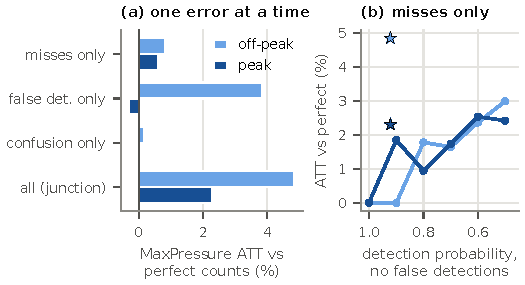
\includegraphics[width=\columnwidth]{figures/camera.pdf}
\caption{MaxPressure under camera errors. (a) Post-hoc: one junction-camera error type at a
time. (b) Only missed vehicles, uniform over classes (lines), against the junction camera at its
effective detection rate ($\star$).}
\label{fig:cam}
\end{figure}

\section{Discussion and Limitations}

\textbf{Why the LLMs match but do not beat MaxPressure.} The hybrid prompt shows each option's
pressure, the information MaxPressure uses; a model that reads it correctly becomes MaxPressure,
as the hosted model did. Small models misread it: with earlier prompts they treated low
pressure as good and kept the current phase, and the prompt fix changed \model{gemma4:e4b} but
not the 3~B models. The guard turns such a model into MaxPressure with noise: the remaining
departures, within \V{cfg.guard.margin}{20}\% of the top pressure, cost a little off-peak. To beat
MaxPressure an agent needs information it lacks or planning over several decisions; neither was
asked of these agents.

\textbf{Why they help ambulances.} Here the agent has information MaxPressure lacks, and one
sentence in the prompt was enough. A hand-written preemption rule did slightly better and is
simpler to verify; the case for an LLM is flexibility, since the same mechanism can carry rules
that are awkward to hard-code (closures, school zones, a late bus). Only ambulances were tested.

\textbf{Limitations.} The camera errors are a \emph{proxy}: measured on dash-camera images, not
on a pole-mounted junction camera, and each snapshot is independent (no tracking). Three seeds
per scenario (five with ambulances) are few and no significance test was run, so differences of one or two percent are within noise. LLM runs are not bit-for-bit repeatable on a GPU, although every
decision is logged and replayable. CityFlow is lane-based and, with lane changing on, not
exactly repeatable; we run with it off, where repeated runs are identical. Demand is synthetic
and steady, the network small, latencies specific to a GTX 1650, and everything is simulation
only: no real signal was controlled. Unlike CoLLMLight we did not fine-tune, so our results
neither confirm nor contradict its claims.

\section{Conclusion and Future Work}

A small local LLM, guided and guarded by MaxPressure, controlled an Indian-mix network within
\V{f.peak.llm.vs_mp}{0.5}--\V{f.off.llm.vs_mp}{0.9}\% of a tuned MaxPressure in real time but
did not improve on it; told about ambulances, it cut their travel time by
\V{e.llm.amb_cut_vs_mp}{31.7}\%, close to a preemption rule, without slowing other traffic.
Measured camera errors cost count-based control a few percent, mostly through false detections,
so a detector's precision matters more than its recall here, and a good fixed plan is a robust
fallback. Future work: agents with memory and tools that plan over several decisions;
fine-tuning small models on simulator feedback; footage from fixed junction cameras with
tracking; larger networks and real demand; and shadow-mode field trials with GPS or V2X
ambulance positions.

\section*{Acknowledgment}
We thank our guide, Dr.\ Mohd Irfan, and the School of Computer Science and Engineering,
VIT-AP University, for their guidance and support. We are grateful to the authors of CoLLMLight,
whose open code made it possible to validate our simulator against theirs; to the CityFlow
developers; and to IIIT Hyderabad and Intel for the India Driving Dataset.

% Balances the last page's columns (column break before this reference); adjust if the
% reference list changes.
\IEEEtriggeratref{26}
\bibliographystyle{IEEEtran}
\bibliography{refs}

\end{document}
